\documentclass{standalone}
\usepackage{tikz}
%\usetikzlibrary{intersections,calc}
\begin{document}

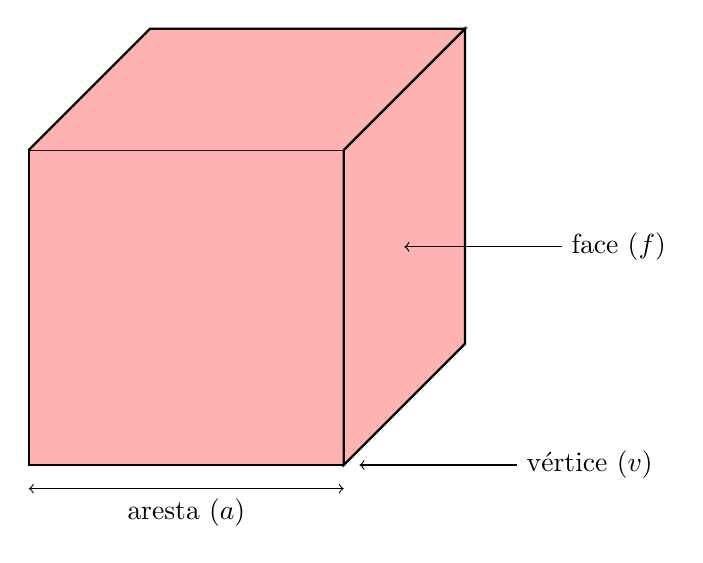
\begin{tikzpicture}
% \draw[help lines,black!30] (-10,-10) grid (10,10);
% \draw[thick,->] (0,-10) -- (0,10) node[left]  {y};
% \draw[thick,->] (-10,0) -- (10,0) node[below] {x};
% \foreach \x in {-10,...,10} \node[left,color=red] at (0,\x) {\x} node[below,color=red] at (\x,0) {\x};
% \node[below right,color=red] at (0,0) {0}; 



   \draw[thick, black, fill=red!30, draw=black] (4,0,0) -- (0,0,0) -- (0,4,0) -- (4,4,0);
   \draw[thick, black, fill=red!30, draw=black] (4,0,0) -- (4,0,-4) -- (4,4,-4) -- (4,4,0) -- cycle;
   \draw[thick, black, fill=red!30, draw=black] (0,4,0)  -- (0,4,-4)  -- (4,4,-4)  -- (4,4,0) ;
   % \draw[style=dashed, color=black] (4,0,-4) -- (0,0,-4)-- (0,4,-4);
   % \draw[style=dashed, color=black] (0,0,0) -- (0,0,-4); 
   \draw[<->](0,-0.3,0)--(4,-0.3,0);
   \draw node[below] at (2,-0.3,0) {aresta ($a$)}; 
   \draw[<-] (4,2,-2) -- +(2,0) node[right]       {face ($f$)};
   \draw[<-] (4.2,0,0) -- +(2,0) node[right] {vértice ($v$)};


           
    % Preenche as faces do cubo
   % \draw[<-] (6,3,0) -- +(2,0,0) node[right]       {aresta ($a$)};
   % Desenha as bordas do cubo
   % \draw[thick,black] (0,0,0) -- (6,0,0) -- (6,6,0) -- (0,6,0) -- (0,0,0);
   % \draw[thick,black] (6,0,0) -- (6,0,-6) -- (6,6,-6) -- (6,6,0);
   % \draw[thick,black] (6,0,-6) -- (0,0,-6) -- (0,6,-6) -- (6,6,-6);
   % \node[fill=red!10] at (3,3,3) {$v + f = a + 2$};
\end{tikzpicture}

\end{document}